\section{Forest Fire Theory}
\subsection{The Fundamentals of Fire}
For there to be a fire, the fire triangle(Showed in figure \ref{fig:fire-triangle}) needs to be satisfied. The three components in the fire triangle is an oxidizing agent, fuel and heat. All these tree depend on each other and without one of them, there will be no fire. An oxidizing agent is a substance that removes an electron from another substance. Oxygen is the normal example of an oxidizing agent.
\begin{figure}[here]
  \centering
      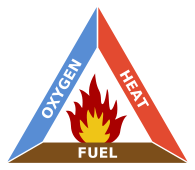
\includegraphics[width=0.65\textwidth]{theory/graphics/fire-triangle.png}
  \caption{ Fire triangle. }
  \label{fig:fire-triangle}
\end{figure}
\subsection{Analyzing the Shape of Fire}
By looking at the shape of a fire, you can determine what part of the fire is a heading fire or a backing fire. Shown in figure \ref{fig:fire-ignition}, the heading fire is much lager then the backing fire, this is due to the fact that heading fire moves more quickly. The reason for this is that a heading fire is always going the same way as the wind, and a backing fire is going in the opposite direction of the wind.
\begin{figure}[here]
  \centering
      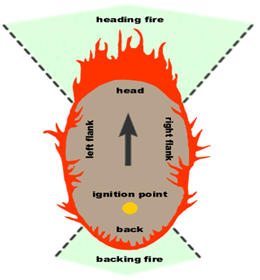
\includegraphics[width=0.65\textwidth]{theory/graphics/fire-ignition.png}
  \caption{ This illustration shows different parts of a fire which is ignited from one point. }
  \label{fig:fire-ignition}
\end{figure}
\subsection{Fire Movement}
The flames tend to move on the uphill side quickly due to the easy access to fuel. Moreover hot convective air from fires moves up the slope drying out fuels which means it will ignite easier as seen in figure \ref{fig:fire-slope}. As a result the fire spreads twice as fast while moving uphill. It is an important fact that fire behavior in complex landscape is unpredictable due to narrow valleys and ridges. As it can suddenly change direction and magnitude. []
\begin{figure}[here]
  \centering
      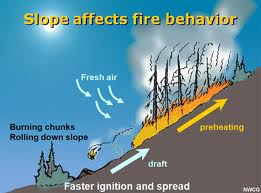
\includegraphics[width=0.65\textwidth]{theory/graphics/fire-slope.jpg}
  \caption{Slope affects fire behavior. [] }
  \label{fig:fire-slope}
\end{figure}
\subsection{Fire Types}
There are different types of fires, surface fire, crown fire and ground fire are tree types of forest fires. The surface, as seen to the left in figure \ref{fig:fire-types}, fire burns on the forest floor and often use shrubs, grass, broken branches, litter and leafs as the source of fuel. When they grow large enough, almost anything will do as fuel. Crown fires, as seen to the right in figure \ref{fig:fire-types}, are always ignited by surface fire, this is the fire in trees or bush tops. Fires on the ground may use subsurface organic material as fuel, these fires may be ignited from surface fire. Soil with a high organic percentage such as peat found in the arctic tundra, bogs and swamps tends to be the fuels to these kinds of fires.
\begin{figure}[here]
  \centering
      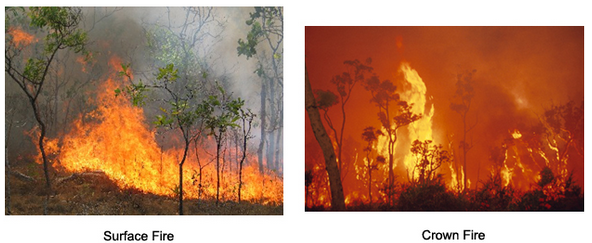
\includegraphics[width=0.65\textwidth]{theory/graphics/fire-types.png}
  \caption{Surface fire and crown fire. [] }
  \label{fig:fire-types}
\end{figure}
\subsection{Wind}
Wind is one of the most important factors in controlling and changing rate and direction of the spread of fire. Figure \ref{fig:fire-wind} shows how the wind changes the direction of fire. As a rule the fire changes direction wherever the wind blows. First the wind direction is from north west, which means the fire spreads south east. After the wind has changed direction the fire follows and now spreads towards north east.
\begin{figure}[here]
  \centering
      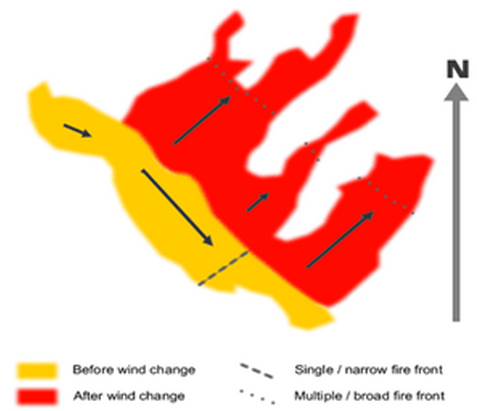
\includegraphics[width=0.65\textwidth]{theory/graphics/fire-wind.png}
  \caption{Wind affects fire. [] }
  \label{fig:fire-wind}
\end{figure}
\subsection{Climate and Vegetation Effect on Fire}
\begin{figure}[here]
  \centering
      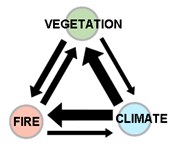
\includegraphics[width=0.65\textwidth]{theory/graphics/fire-climate.png}
  \caption{Climate, vegetation and fire create a chain as follows: [] }
  \label{fig:fire-climate}
\end{figure}
As illustrated in figure \ref{fig:fire-climate} climate has a strong influence on vegetation and fire. This is illustrated by the thickness of the arrows . For instance climate has a far-reaching effect on vegetation type, while vegetation and fire has a small effect on the climate. The climate has a big impact on the vegetation. For example a tropical rain forest is a result of high humidity and high temperatures. If we remove the high humidity savannah and grassland will appear. Fire will occur when the weather is hot, dry, windy, lightning or low humidity. With all these conditions in place in addition of a temperature rise the chances of an intense fire is present. On the other hand fire would rarely occur if precipitation and the moisture in the fuel is high.  Moreover fire has a huge influence on vegetation type, it can be damaging to the vegetation in rain forests because it has problems with the extreme changes. Similarly vegetation can affect fire. Some plants has a high level of moisture while others can be dry. This difference in flammable degree can have a noticeable impact on how the fire spreads and makes it harder to predict how the spread will be.
\subsection{Temperature and Flame Height}
The temperature of a forest fire depends on some conditions like climate and type of fuel. An average forest fire have a temperature up to $800^{\circ}C$, and a flame height up to 1 meter. In some extreme cases the temperature can exceed $1200^{\circ}C$ and flame heights can become over 50 meters. The higher flames are, the more crown fires will occur during a forest fire.
\subsection{Relative Humidity}
Relative humidity have a huge impact on water content in small fuel sources as water vapor can easily penetrate into or escape from the center of small fuel sources. Thus wood with a high amount of water content will ignite more slowly compared to dry wood. The reason for this is that the water inside of the wood needs to vaporize before the wood can burn, and the vaporization of this water may require a lot of energy. In addition, high water content will cause a fire to burn with a lower intensity as the water has to vaporize before the fire can reach its maximum intensity [].
\subsection{Rate of Spread}
The time it takes for a fire to move over a horizontal distance is the Rate of Spread. Since the rate of fire may vary a lot from any point the fire is spreading, it is usually an average value. The head fire will have the highest rate of spread, the back fire will have the lowest and the flanking fire will have a medium rate of spread. An easy way to measure the rate of fire is to find two or more landmarks of a known distance from each other, then take the time for the fire to pass the landmarks. There are also other techniques that can be used to measure the rate of spread, like using a video camera or placing firecrackers [].
\begin{figure}[here]
  \centering
      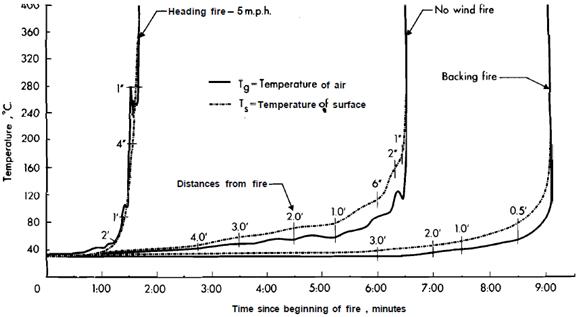
\includegraphics[width=0.9\textwidth]{theory/graphics/fire-prediction.jpg}
  \caption{Mathematical Model for predicting fire spread in forest fire. [] }
  \label{fig:fire-prediction}
\end{figure}
\subsubsection{Formula to calculate rate of spread}
Rothermel’s equation have been the basis for most of the fire spread prediction models. One formula to calculate the rate of spread was mathematically expressed by this equation. This equation as shown in figure \ref{fig:fire-prediction}, is the heat received by the fuels ahead of the fire divided by the heat required to ignite the fuels.
\begin{equation}
R=\dfrac{IR \xi(1 + \Phi W + \Phi S)}{\rho \eta \varepsilon  Qig}
\label{eq:fire-spreadd}
\end{equation}
\begin{itemize}
\item $ R $ = rate of spread of the flaming front
\item $IR$ = reaction intensity
\item $\xi$ = proportion of the reaction intensity that heats adjacent fuel particles to ignition
\item $\Phi W$ = dimensionless multiplier accounting for the effect of wind in increasing the proportion of heat that reaches adjacent fuels
\item $\Phi S$ = dimensionless multiplier accounting for the effect of slope in increasing the proportion of heat that reaches adjacent fuels
\item $\rho \eta$ = ovendry fuel per cubic foot of fuel bed (lb/ft)
\item $\varepsilon$ = dimensionless number accounting for the proportion of a fuel particle that is heated to ignition temperature at the time flaming combustion starts (near unity for fine fuels and decreases toward zero as fuel size increases)
\item $Qig$ = heat of pre-ignition, or the amount of heat required to ignite one pound of fuel (Btu/lb)
\end{itemize}
This formula can be used to properly describe rate of spread. This could later be used in combination with other factors, such as wind direction and terrain to correctly implement fire behaviour.
